%%%%%%%%%%%%%%%%%%%%%%%%%%%%%%%%%%%%%%
  %%%%%%%%%%%%%%%%%%%%%%%%%%%%%%%%%%%%%%
  % Do not edit the TeX file your work
% will be overwritten.  Edit the RnW
% file instead.
%%%%%%%%%%%%%%%%%%%%%%%%%%%%%%%%%%%%%%
  %%%%%%%%%%%%%%%%%%%%%%%%%%%%%%%%%%%%%%
  
  
      



\begin{knitrout}
\definecolor{shadecolor}{rgb}{0.969, 0.969, 0.969}\color{fgcolor}\begin{figure}[!h]

{\centering 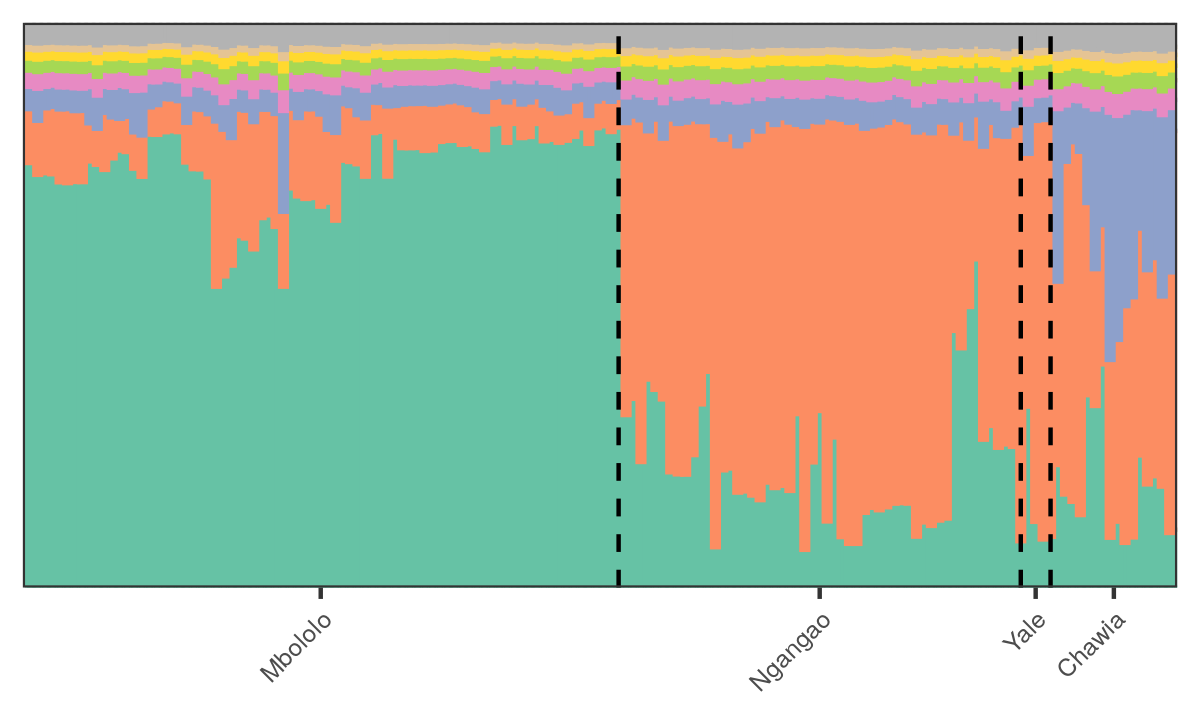
\includegraphics[width=0.98\linewidth,height=0.588\linewidth]{figure/stru_init_fit-1} 

}

\caption[structure initial fit ]{structure initial fit }\label{fig:stru_init_fit}
\end{figure}


\end{knitrout}

    
    

\begin{knitrout}
\definecolor{shadecolor}{rgb}{0.969, 0.969, 0.969}\color{fgcolor}\begin{figure}[!h]

{\centering 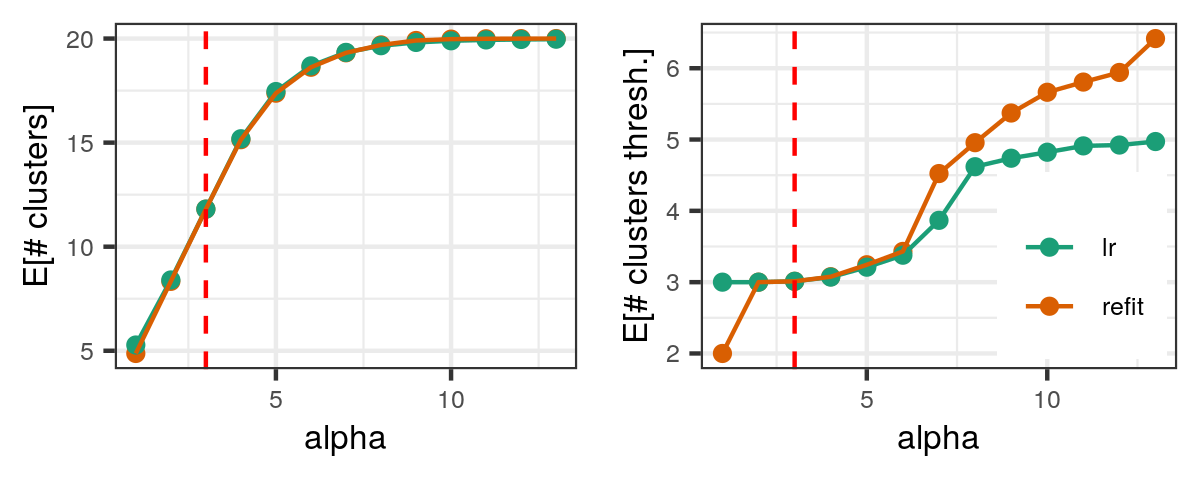
\includegraphics[width=0.98\linewidth,height=0.392\linewidth]{figure/stru_alpha_nclusters-1} 

}

\caption[structure alpha sensitivity]{structure alpha sensitivity: number of clusters }\label{fig:stru_alpha_nclusters}
\end{figure}


\end{knitrout}




\begin{knitrout}
\definecolor{shadecolor}{rgb}{0.969, 0.969, 0.969}\color{fgcolor}\begin{figure}[!h]

{\centering 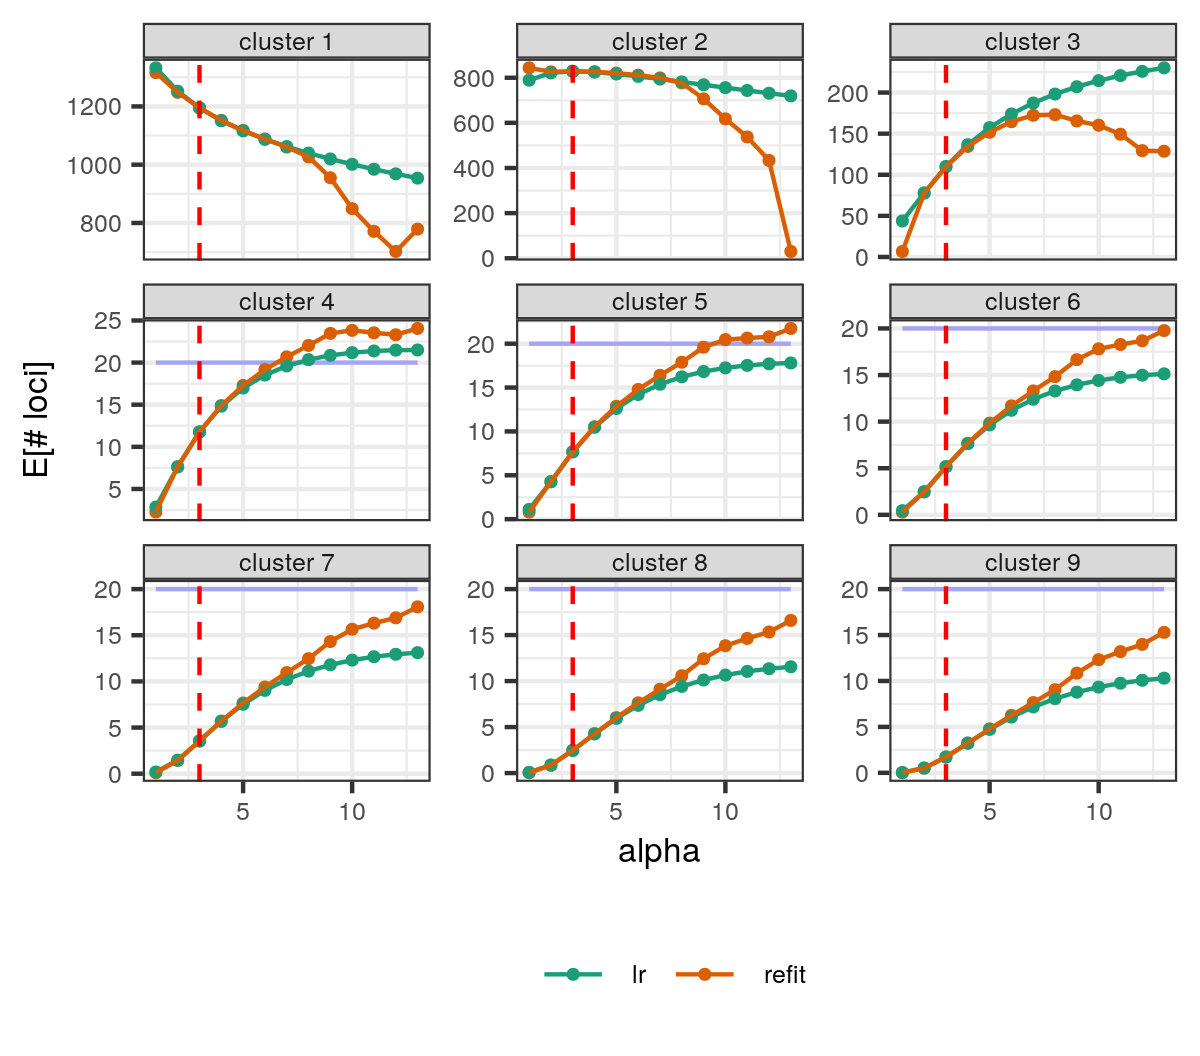
\includegraphics[width=0.98\linewidth,height=0.862\linewidth]{figure/stru_alpha_cluster_weights-1} 

}

\caption[structure alpha sensitivity]{structure alpha sensitivity: cluster weights }\label{fig:stru_alpha_cluster_weights}
\end{figure}


\end{knitrout}



\begin{knitrout}
\definecolor{shadecolor}{rgb}{0.969, 0.969, 0.969}\color{fgcolor}\begin{figure}[!h]

{\centering 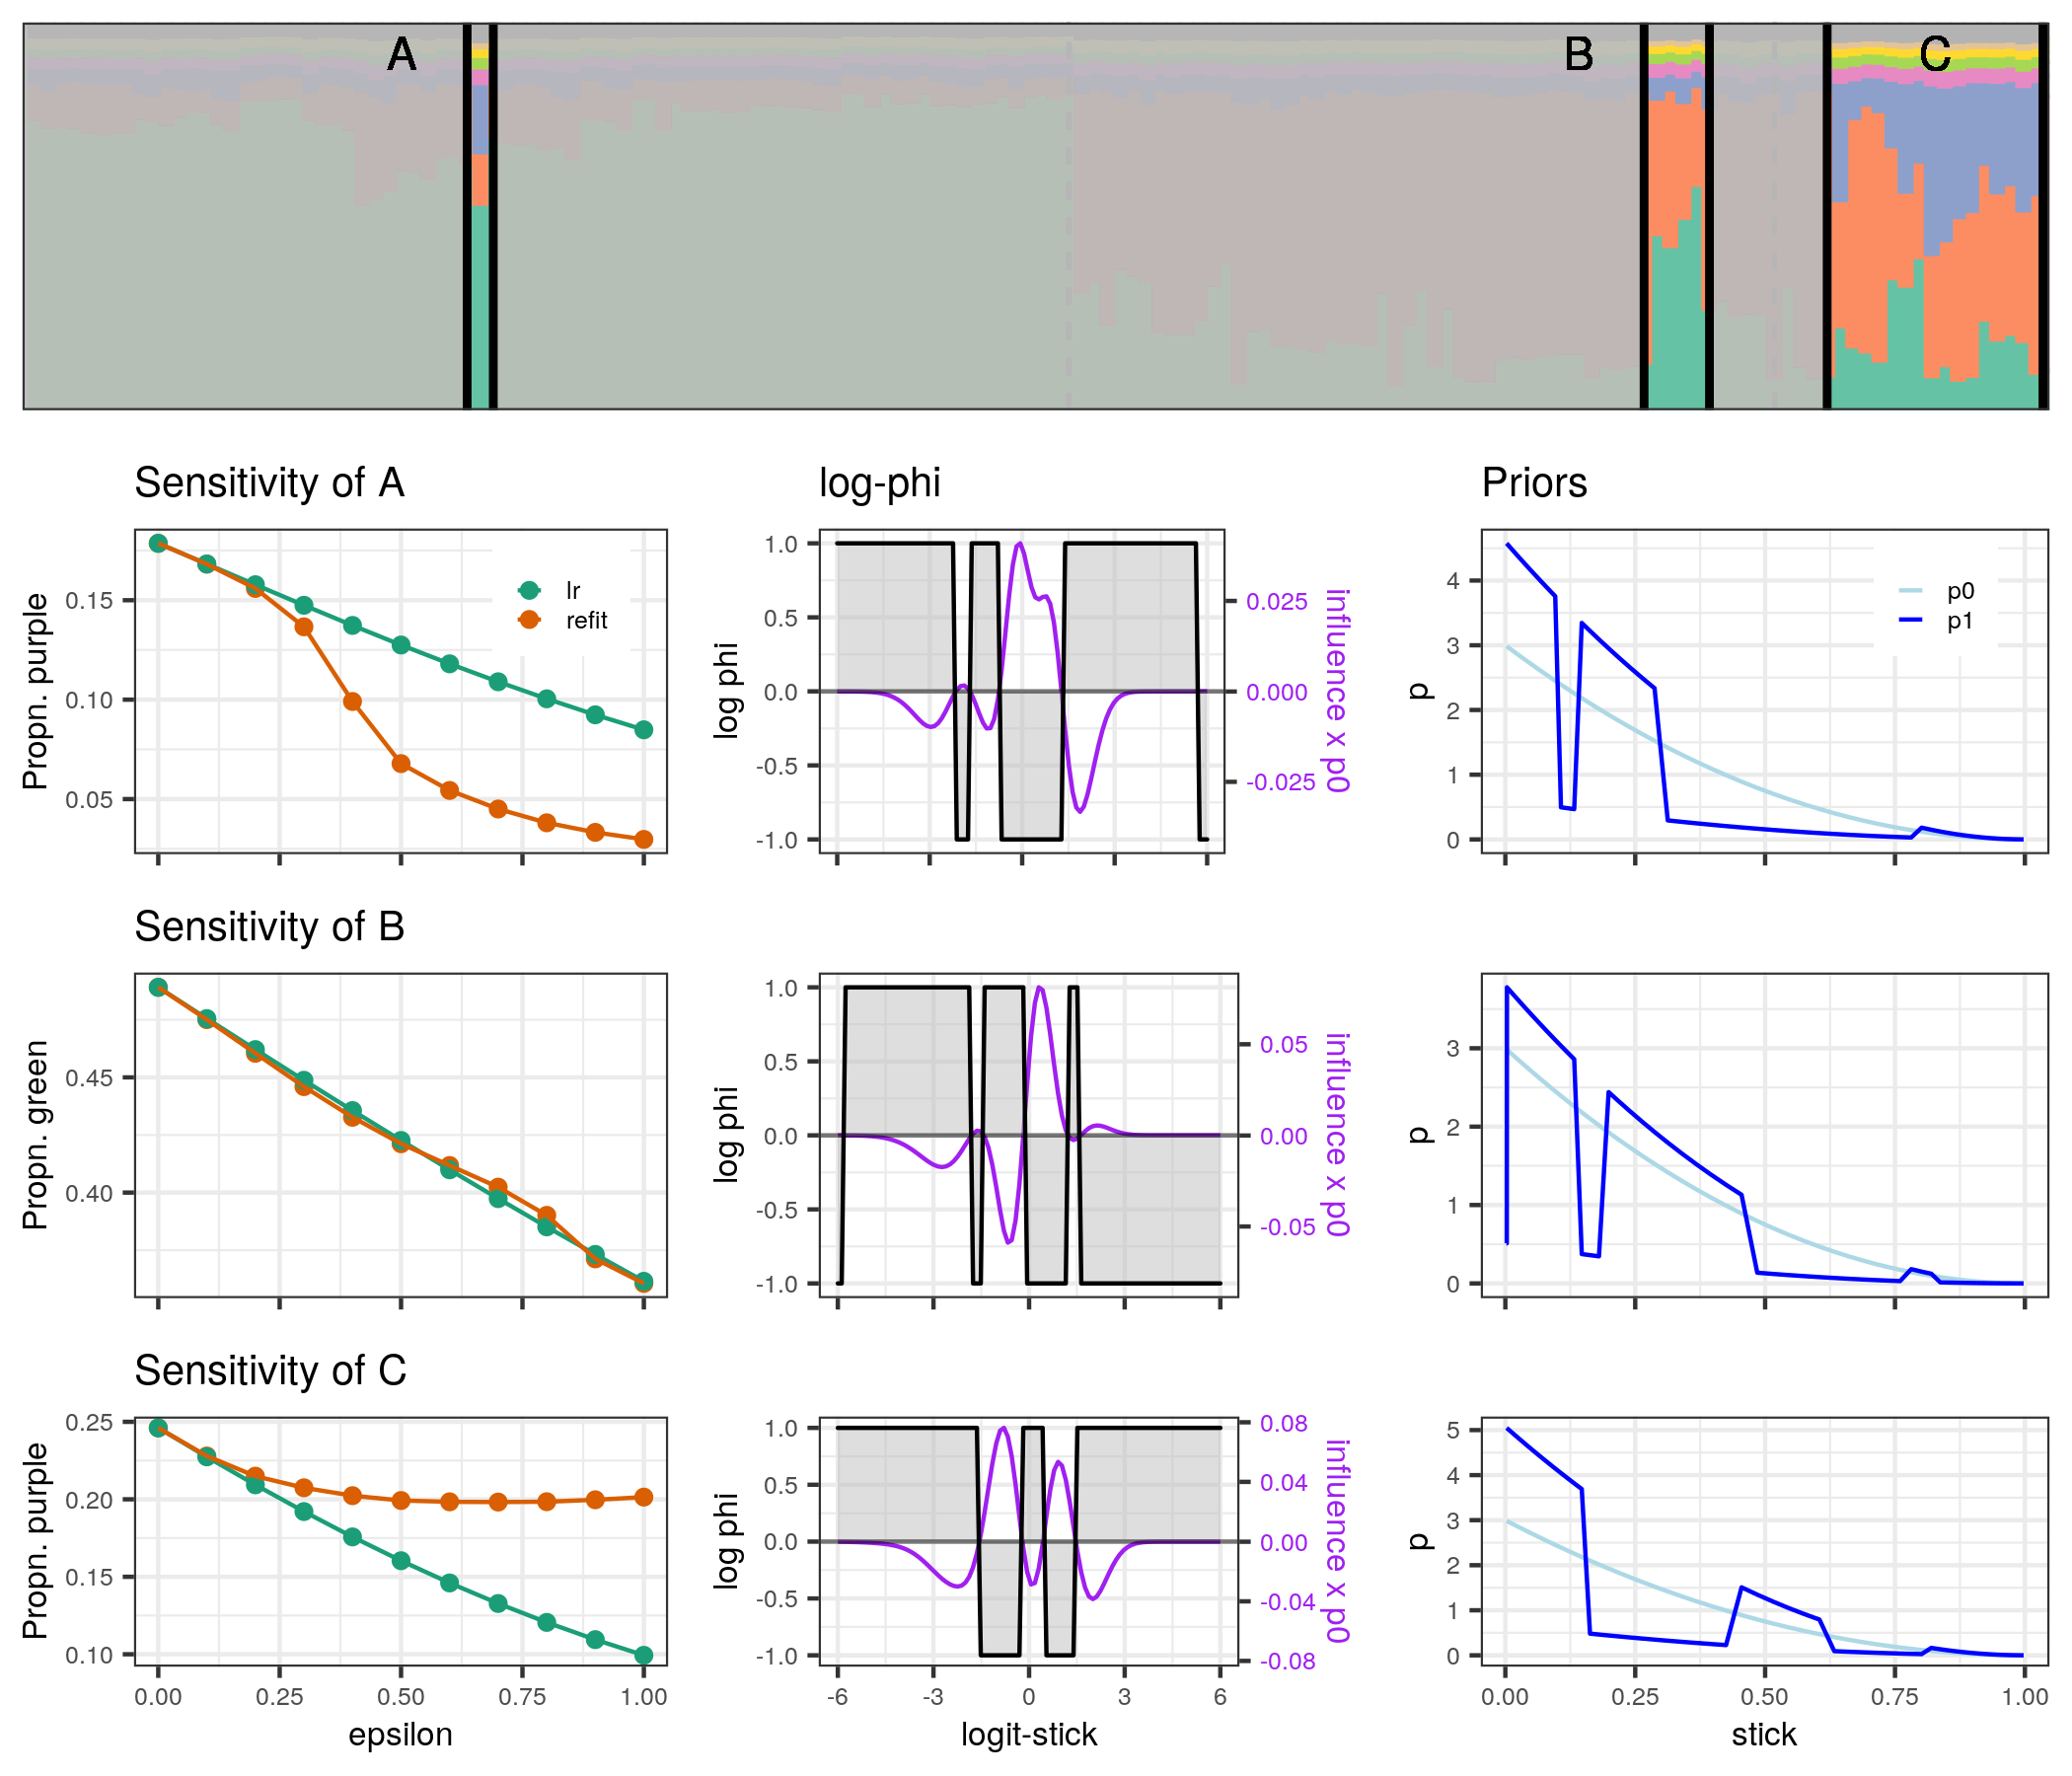
\includegraphics[width=0.98\linewidth,height=1.019\linewidth]{./R_scripts/structure/figures_tmp/fsens_structure} 

}

\caption[structure functional sensitivity ]{structure functional sensitivity }\label{fig:stru_func_sens}
\end{figure}


\end{knitrout}

